\chapter{Implementation - Areas of Application}
\label{ch:impl_aoa}


\section{Manual editing (predefined structures)}
\label{sect:manual_editing}

	The first and foremost use case for Graphinius is simply to be able to interactively build, mutate, and visualize graphs in the browser. Although the final Graphinius Platform will feature a full-blown code editor with code completion and online documentation, the basic functionality can be demonstrated even using a form of REPL every modern browser is automatically equipped with: the debugging console.

	\subsection{Build a graph manually}
	\label{ssect:build_graph_manually}
	
	As depicted in the following Figure, the basic case is to create a new graph structure, add some nodes and edges, and then run different computations on it:
	
	\begin{figure}[H]
		\begin{center}
			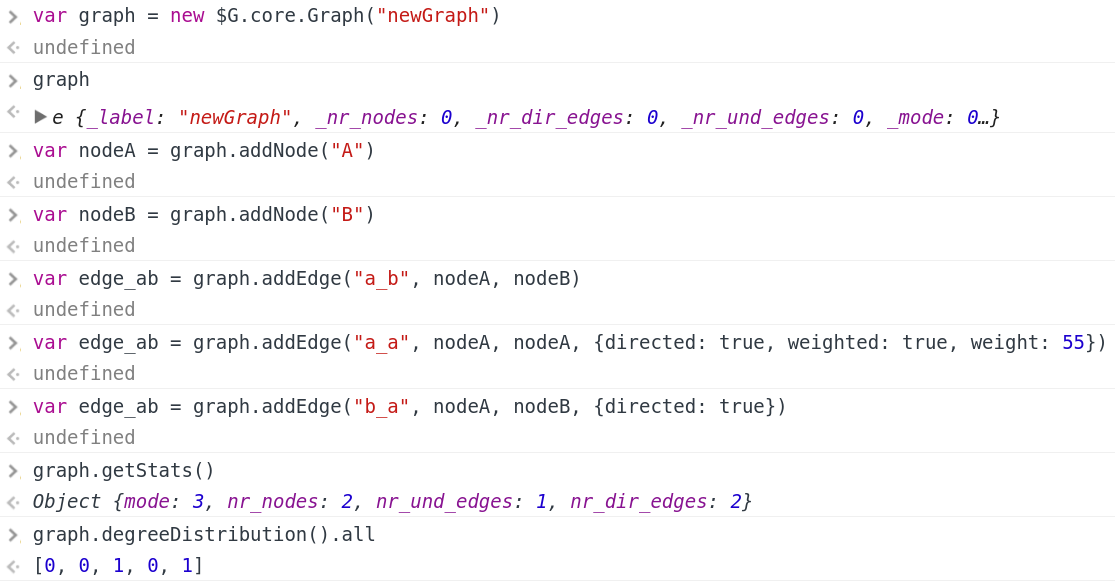
\includegraphics [width=1\textwidth] {figures/buildGraphManually}
			\caption{Manually building a new graph in the console}
			\label{fig:build_graph_manually}
		\end{center}
	\end{figure}
	
	
	\subsection{Load predefined graph and visualize}
	\label{ssect:load_graph}
	
	Using either the CSV or JSON Reader build into GraphiniusJS, we can also request to instantiate a graph from a remote file. Here we use the JSON Reader to load a graph depicting a nevus and render it using GraphiniusVIS:
	
	\begin{figure}[H]
		\begin{center}
			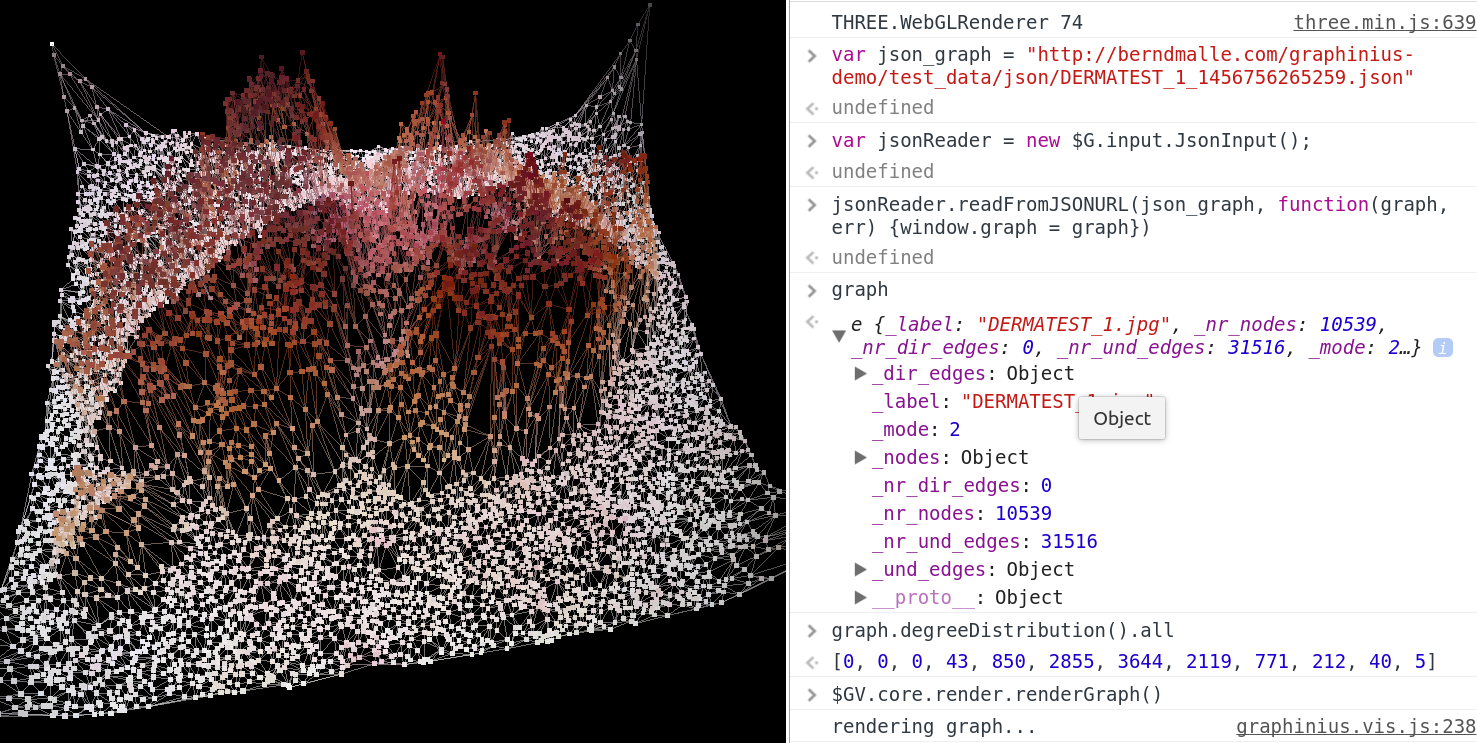
\includegraphics [width=1\textwidth] {figures/loadingGraphInREPL}
			\caption{Loading a JSON graph and visualizing it via the browser console; then determining its degree distribution.}
			\label{fig:load_graph_repl}
		\end{center}
	\end{figure}
	
	
	\subsection{Run a BFS alorithm and visualize}
	\label{ssect:run_bfs_visualize}
	
	After loading a (undirected) graph according to the previous section, we choose a random start node and invoke a breadth-first-search algorithm resulting in a \textit{distance map} centering around that node. The following lines of code show distances and parents of a selection of nodes (note the parent / distance chain...) while the accompanying visualization colors the graph according to the obtained distances via gradient computations (the start node being colored green and the node with maximum distance being colored red).
	
	\begin{figure}[H]
		\begin{center}
			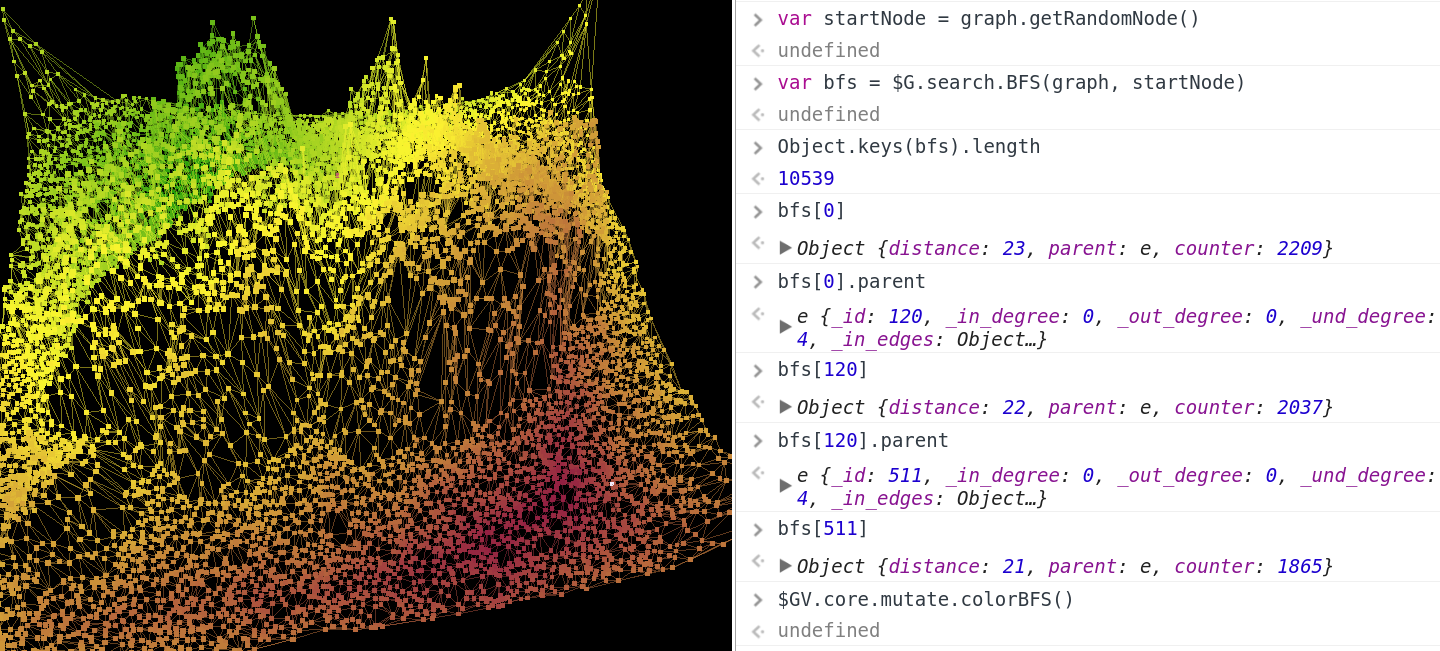
\includegraphics [width=1\textwidth] {figures/colorBFSREPL}
			\caption{Computing a BFS in a live browser REPL \& visualizing the result.}
			\label{fig:color_graph_bfs}
		\end{center}
	\end{figure}
	
	
	\subsection{Run a DFS alorithm and visualize}
	\label{ssect:run_dfs_visualize}
	
	Lastly, we load the same graph as before, this time interpreted as a directed graph, choose a random start node again and invoke a DFS algorithm. This returns to us an array of graph segments representing the node sets reachable from each start node of a respective DFS Visit run (had we chosen an undirected graph, there would only be a single segment). We then output the size of each segment and again visualize the result, assigning to each segment a different color.
	
	\begin{figure}[H]
		\begin{center}
			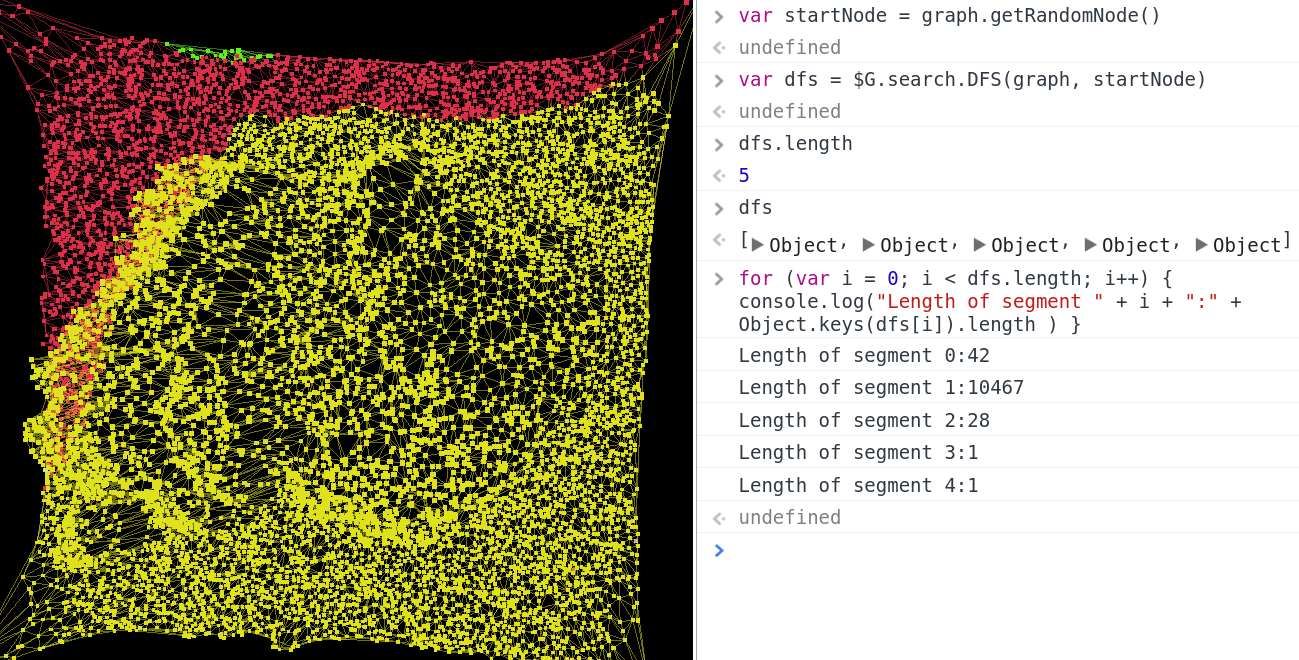
\includegraphics [width=1\textwidth] {figures/colorDFSREPL}
			\caption{Computing a DFS in a live browser REPL \& visualizing the result.}
			\label{fig:color_graph_dfs}
		\end{center}
	\end{figure}	


\section{Graph extraction from images (graphs in preprocessing)}
\label{sect:graph_ext}

	\begin{enumerate}
		\item \textbf{Input image}
		\item \textbf{Image preprocessing}
		\item \textbf{graph based segmentation}
		\item \textbf{visualization}
	\end{enumerate}
	
	\begin{figure}[H]
		\begin{center}
			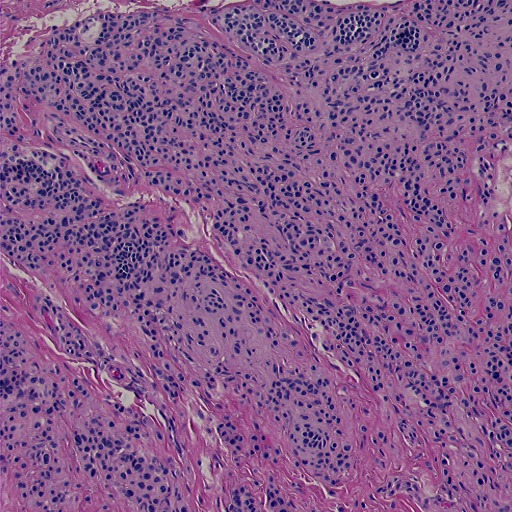
\includegraphics [width=0.24\textwidth] {figures/kruskal/sample2_input}
			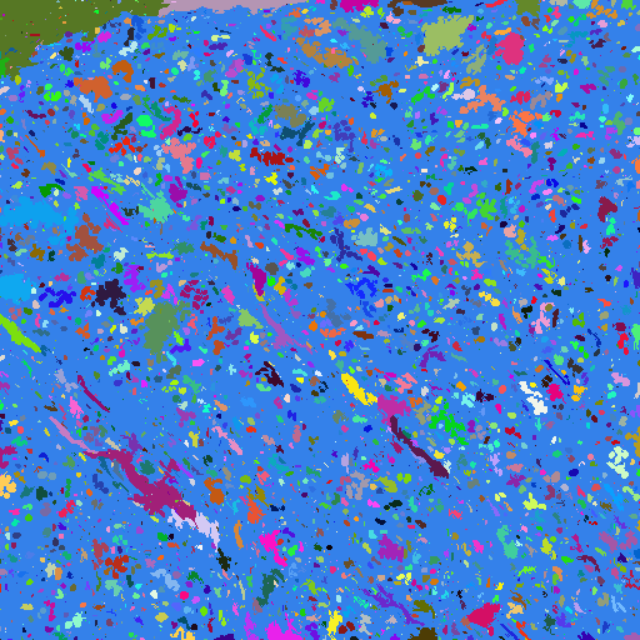
\includegraphics [width=0.24\textwidth] {figures/kruskal/out_rm_01}
			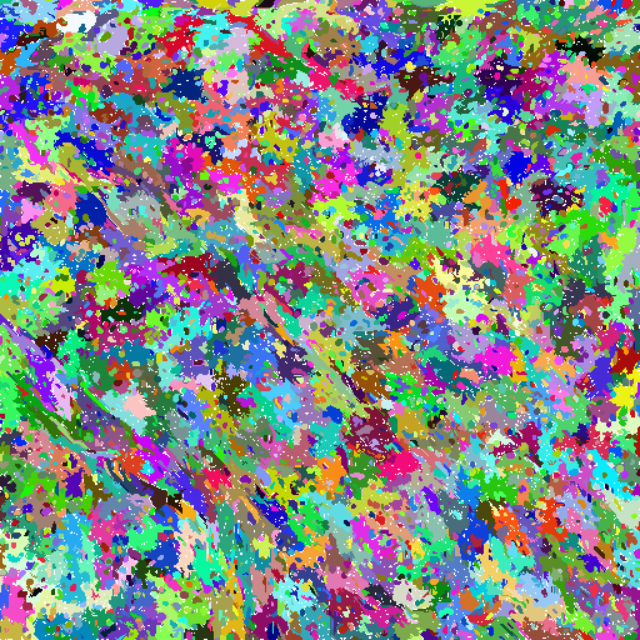
\includegraphics [width=0.24\textwidth] {figures/kruskal/out_rm_02}
			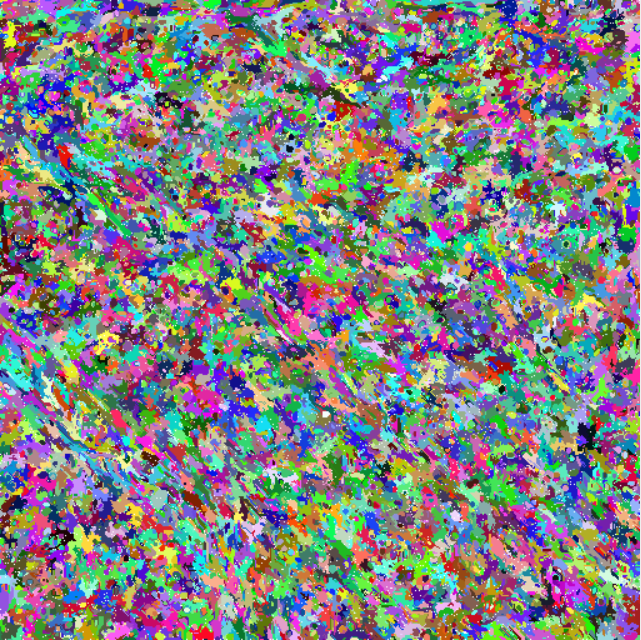
\includegraphics [width=0.24\textwidth] {figures/kruskal/out_rm_03}
			\caption{Kruskal MST based region merging}
		\end{center}
		\small 
		Result of applying a Kruskal based region merging algorithm to an image of numerous small scale regular structures. (1) Input image, (2) Result with parameters $k=1150, s=0, m=\infty$, (3) Result with parameters $k=150, s=5, m=500$, (4) Result with parameters $k=50, s=2, m=150 $.
		
	\end{figure}


\section{Anonymity: SaNGreeA (with iML)}
\label{sect:anonymization}

	\begin{enumerate}
		\item \textbf{Process input data into suitable structure}
		\item \textbf{Enhance structure with graph information (random)}
		\item \textbf{Anonymize via SaNGreeA}
		\item \textbf{prepare individual cost function via iML}
		\item \textbf{Anonymize via SaNGreeA modified}
		\item \textbf{Compare results}
	\end{enumerate}
	
	\begin{figure}[ht]
		\label{fig_anonIML}
		\begin{center}
			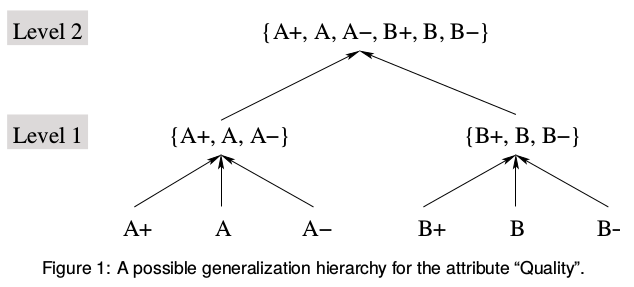
\includegraphics[width=0.8\textwidth]{figures/anonym/gen_hierarchy}
			\caption{Example of a typical generalization hierarchy}
		\end{center}
	\end{figure}	
	
	\begin{figure}[ht]
		\label{fig_anonIML}
		\begin{center}
			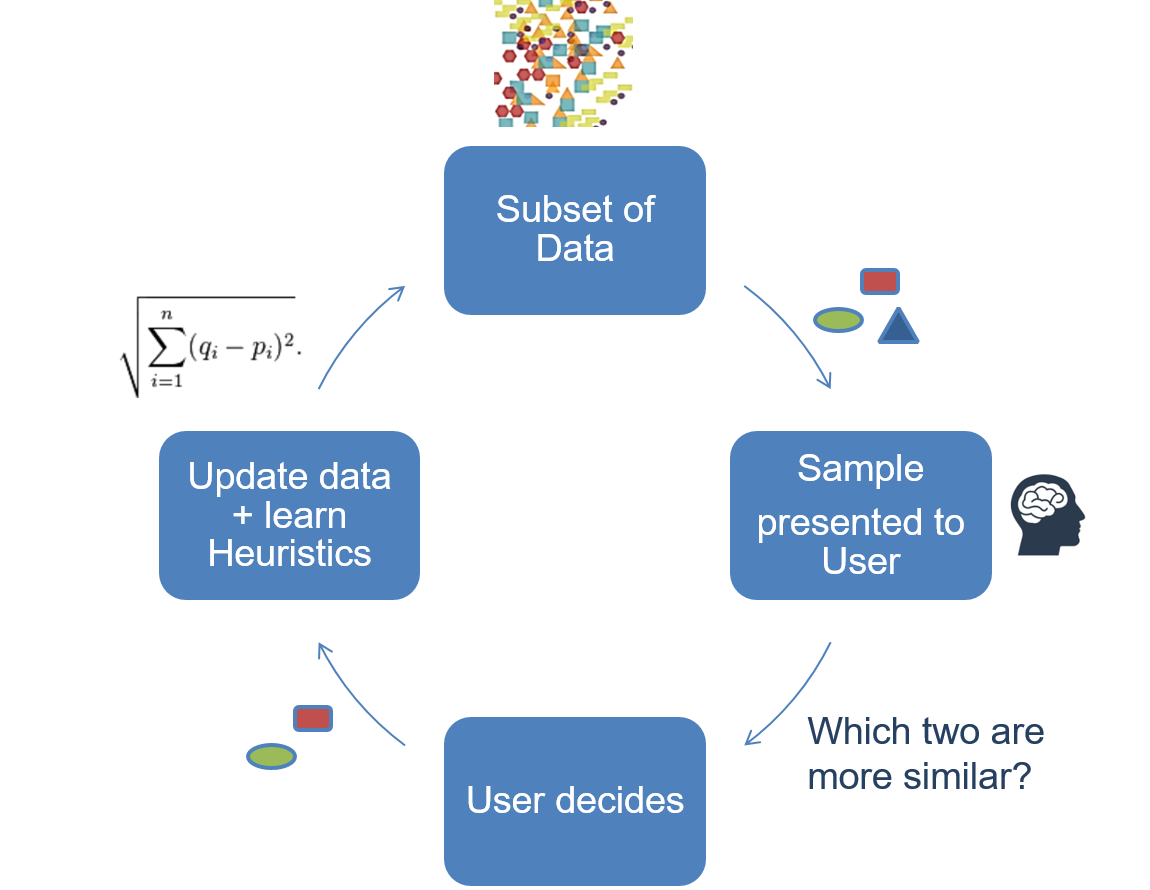
\includegraphics[width=1\textwidth]{figures/anonym/anonIML}
			\caption{Anonymization augmented by IML (human in the loop)}
		\end{center}
	\end{figure}


%\section{NLP: Community extraction \& group labeling (OPTIONAL !!)}
%\label{sect:nlp_community}
%
%	\begin{enumerate}
%		\item \textbf{Import and preprocess free text}
%		\item \textbf{Vectorize text in trigram feature space}
%		\item \textbf{Compute similarity kernel matrix}
%		\item \textbf{Extract connectivity graph from kernel matrix}
%		\item \textbf{Identify and extract communities from graph (SCC analysis?)} - node types
%		\item \textbf{Apply group labels to free text elements} - group labeling / node coloring
%	\end{enumerate}

